\documentclass[11pt,a4paper]{article}
\usepackage[margin=24mm]{geometry}\usepackage{fontspec,unicode-math,booktabs,graphicx,hyperref}
\setmainfont{STIXGeneral}\setmathfont{STIX Two Math}\hypersetup{hidelinks}
\title{Two additional complete-manuscript comparisons}
\author{Human Compression Project}\date{11 October 2026}
\begin{document}\maketitle
These are two separate topics, each with a complete common paper and one complete application. The originals are Piedade's \emph{Infinite Families of Hypertopes from Centrally Symmetric Polytopes} (F015, final EJC edition, 21 pages), and Buekenhout--Leemans--Tranchida's \emph{A new algorithm to classify chiral polytopes with a given automorphism group} (L028, revised ULB author edition, 14 pages). The 64 detailed records describe these two accepted principal contracts; they are not 64 manuscripts. The earlier ten-topic, 27-original report is unchanged.

\paragraph{Whole topics and conditional applications.}
The primary unit is calibrated NFC characters excluding whitespace. Every authored page is included: front matter, references, source software and extractable diagram and table text remain. Only exact repeated page furniture is removed.
\begin{center}\begin{tabular}{lrrrr}\toprule
Topic & Original & Common & Application & Printed code\\\midrule
Matching (F015) & 37,951 & 16,732 & 17,168 & 4,998 \\
Chiral enumeration (L028) & 29,599 & 8,831 & 23,171 & 11,940 \\
\bottomrule\end{tabular}\end{center}
For each topic, let $L$ be the complete original, $U$ the whole common paper, $A$ the complete application, and $P$ the entire accompanying program bundle. We report
\[
 R_{\rm written}=\frac{c(L)}{c(U)+c(A)},\qquad
 r\mid(U,P)=\frac{c(L)}{c(A)}.
\]
The second comparison assumes that \emph{all of $U$ and all of $P$ have already been acquired}. It is not a whole-topic saving. Shared material is fully charged independently in each topic.
\begin{center}\begin{tabular}{lrrrr}\toprule
Topic & Whole written & Conditional & With printed code & With raw code\\\midrule
Matching & 1.119 & 2.211 & 0.976 & 0.991 \\
Chiral enumeration & 0.925 & 1.277 & 0.674 & 0.687 \\
\bottomrule\end{tabular}\end{center}
Matching is shorter as a complete written replacement in this unit, but slightly longer when its full code is included. Chiral enumeration is longer as a complete topic in this coordinate. Both individual applications are shorter once the full common acquisition has been paid. A factor below one means that the replacement costs more in the stated coordinate.

The complete raw program costs are 4,408 for Matching and 11,090 for chiral enumeration. Printed and raw software are alternative representations; they are never added together. Matching's exceptional-orbit GAP census is a finite proof premise. All three chiral programs are retained in full: reference enumeration, formula evaluation and independent involution-count validation. They do not replace the uniform written proof. Three operational drivers and two Lean files are inventoried separately; the fourteen Lean declarations do not establish end-to-end formalization.
\newpage
\begin{center}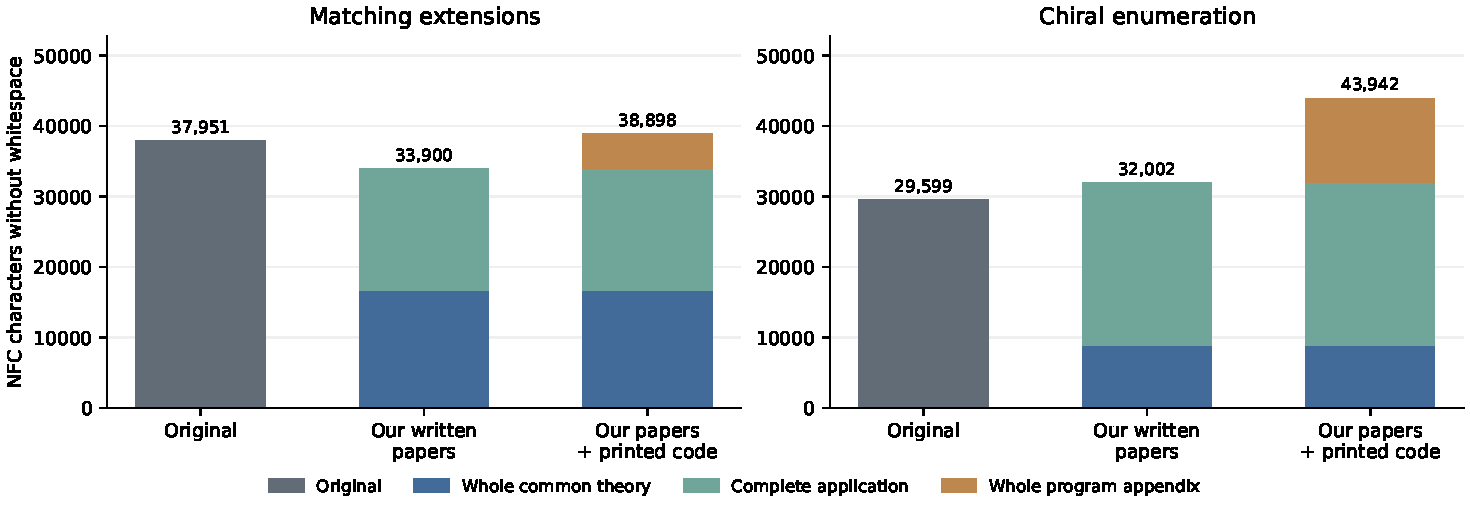
\includegraphics[width=\textwidth]{whole_costs.pdf}\end{center}
The bars charge the full common paper and application, followed by the complete program appendix where shown. There is only one application in each new topic; this does not establish a recurring sawtooth pattern or a minimum proof complexity.

\paragraph{Unit sensitivity.}
For calibrated selected text with NFC normalization:
\begin{center}\begin{tabular}{lrrrr}\toprule
 & \multicolumn{2}{c}{Matching} & \multicolumn{2}{c}{Chiral enumeration}\\
Unit & Whole & Conditional & Whole & Conditional\\\midrule
Whitespace tokens & 1.140 & 2.262 & 1.003 & 1.391 \\
Alphanumeric runs & 1.290 & 2.531 & 1.123 & 1.547 \\
Nonspace characters & 1.119 & 2.211 & 0.925 & 1.277 \\
Collapsed-space characters & 1.123 & 2.219 & 0.938 & 1.296 \\
Collapsed-space UTF-8 bytes & 1.113 & 2.200 & 0.979 & 1.354 \\
\bottomrule\end{tabular}\end{center}
The exact data retain all five units under NFC and NFKC for raw untrimmed, raw selected and calibrated selected text: 30 coordinates per topic and 240 fractions. Raw untrimmed counts keep page furniture on both sides. These alternatives matter: chiral enumeration is slightly shorter in whitespace tokens, but longer in nonspace characters and UTF-8 bytes. No unit-independent compression conclusion is asserted.

\paragraph{Scope, attribution and unknown costs.}
F015's intended finite families, defining presentations, orders and halved geometries are recovered with the accepted corrections. The printed 120-cell presentations omit twenty unordered-pair orbits and define infinite groups; the repaired finite presentations are kept distinct. The original extension/lattice theorem and stated toroid-coordinate descriptions remain attributed inputs. Incidental catalogue comparisons are excluded from the recovered principal contract, while their text remains in the whole-source numerator.

L028's complete connected chiral enumeration covers every finite input group and all ranks. Oriented and unrooted classes are distinguished; duality is not quotiented. The geometric reconstruction and almost-simple involution estimate remain attributed inputs. Source timings remain empirical observations. Corrected table entries and the regular-output qualification do not create an additional source or an open-question solution.

Full retained external proofs, unprovided historical software, graphic layout and complete formalization remain unknown, not zero. The source PDFs contain vector mathematical content; this text comparison does not price its complete visual information. The independently accepted input audit covers 68 pages, 240 PDF and 90 raw-file cells, 78 actual Type1 dictionaries and 1,358 glyph classes. Its 660 repairs preserve visible components. A code-wrap hook without an asserted exact Unicode equivalent retains its literal extracted comma, an explicit UTF-8 representation limitation. No source mathematics is rewritten by calibration.

This numerical packet requires distinct arithmetic, plot and reader review. It adds no mathematical or conjecture credit and does not alter the existing scientific contracts or earlier measurements.
\end{document}
